\chapter*{Appendices}
\addcontentsline{toc}{chapter}{Appendices}

\section*{The Gantt Chart for Task Schedule}
\addcontentsline{toc}{section}{The Gantt Chart for Task Schedule}
\begin{figure}[H]
    \centering
    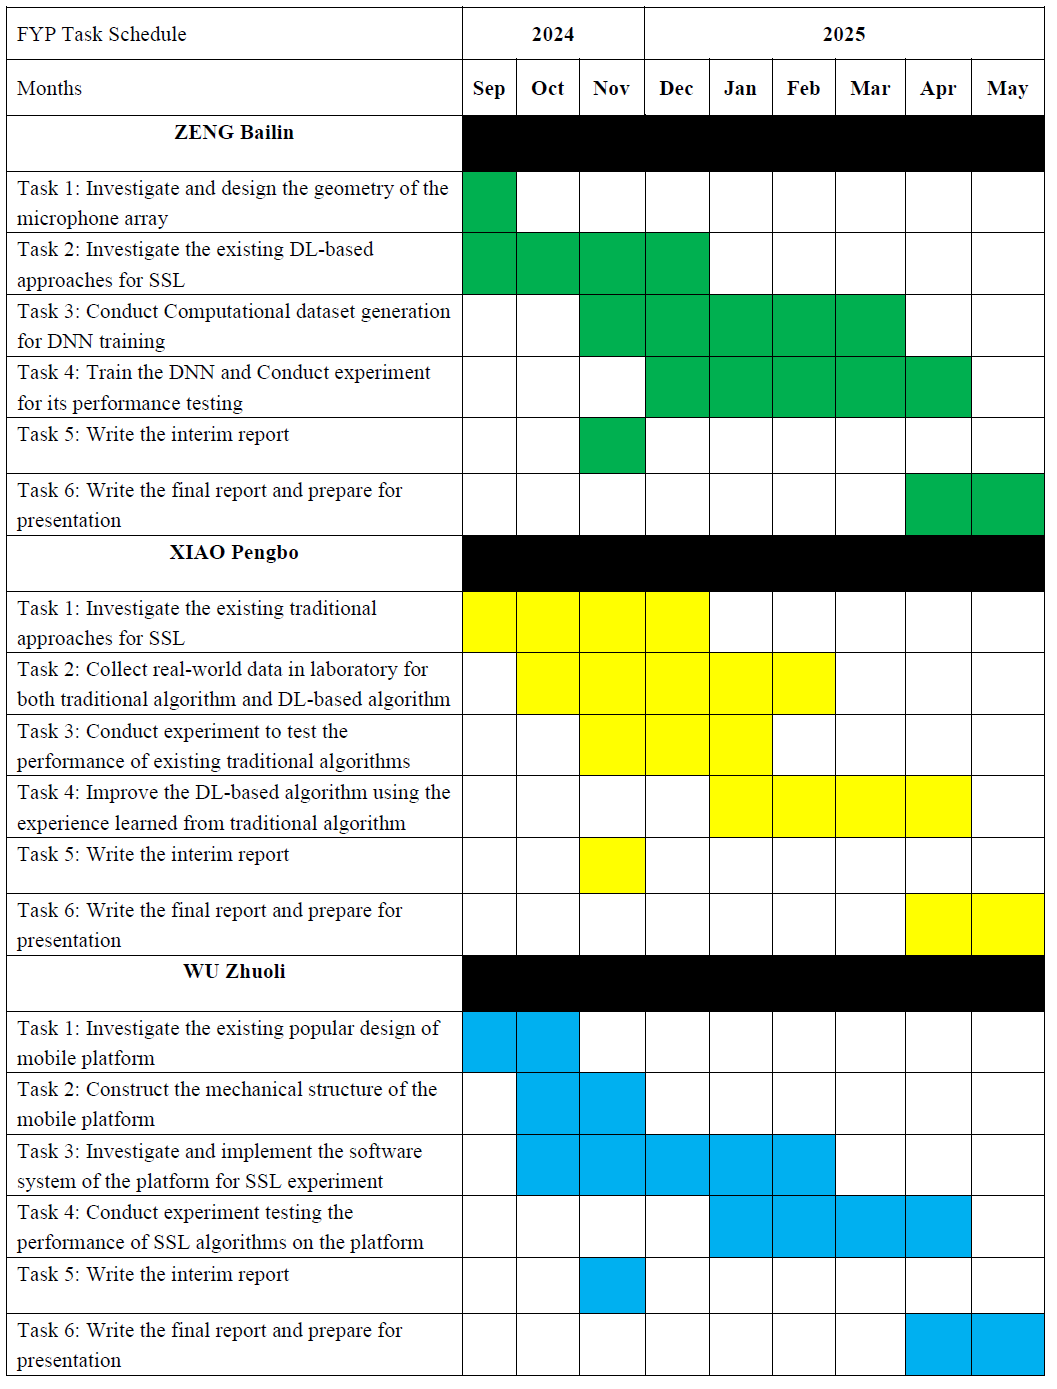
\includegraphics[width=1\linewidth]{figures/Gantt_chart.png}
\end{figure}



\section*{The DL Experiment Result of Different Batch Sizes}
\addcontentsline{toc}{section}{The Experiment Result of Different Batch Sizes}
\begin{figure}[H]
    \centering
    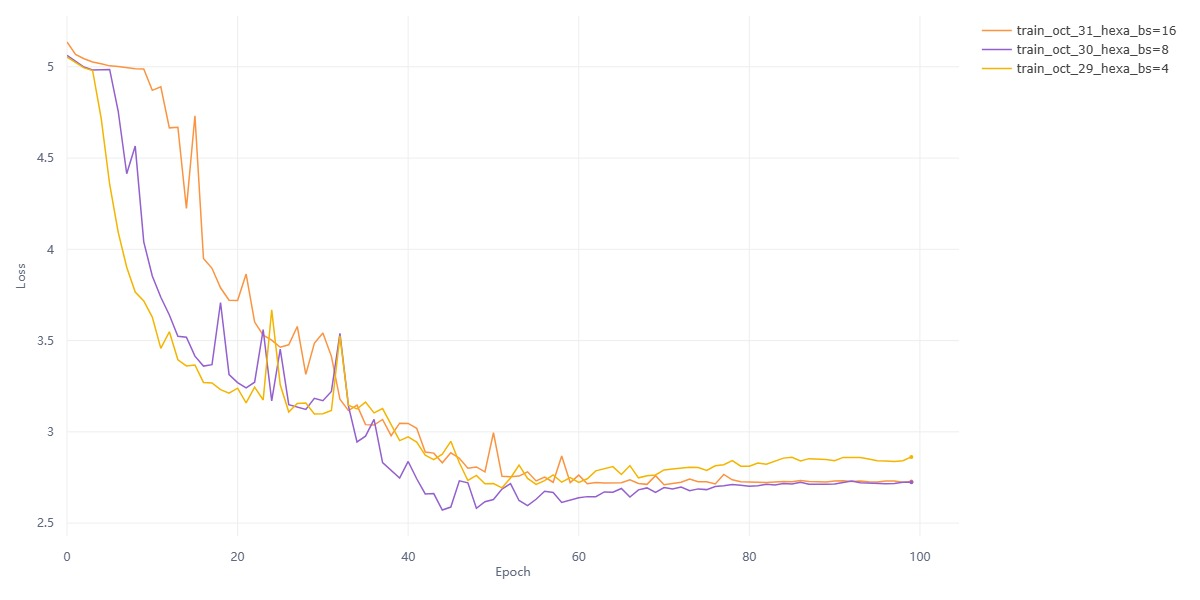
\includegraphics[width=1\linewidth]{figures/BS Valid_ Loss VS epoch.jpeg}
    \caption{Validation: Loss vs Epoch for Different Batch Sizes}
\end{figure}
\begin{figure}[H]
    \centering
    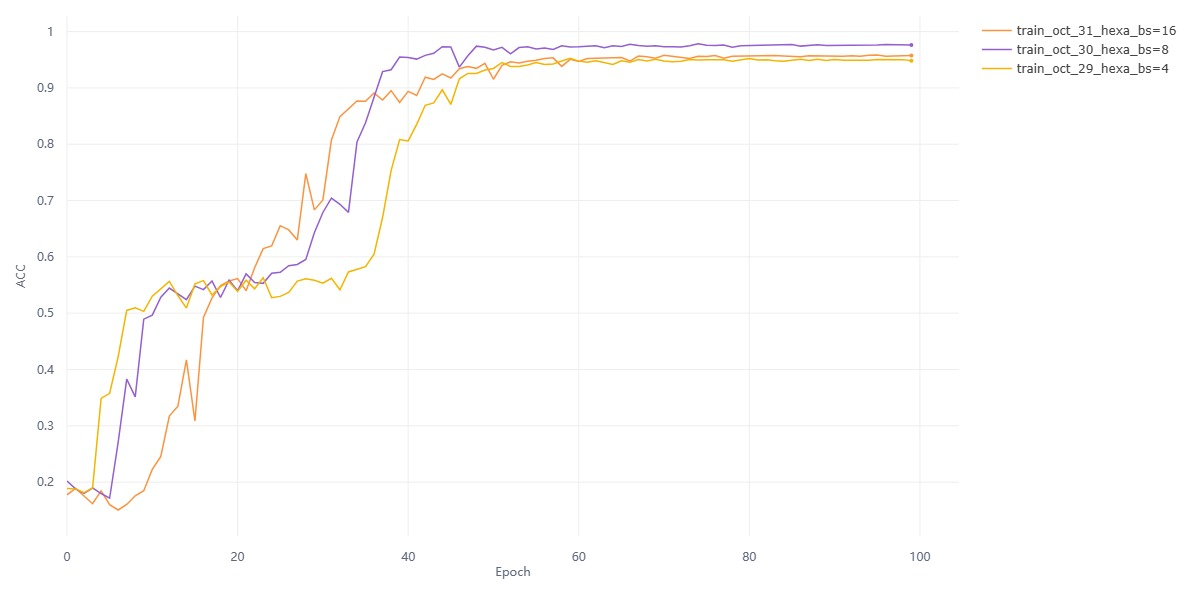
\includegraphics[width=1\linewidth]{figures/BS Valid_ ACC VS epoch.jpeg}
    \caption{Validation: ACC vs Epoch for Different Batch Sizes}
\end{figure}
\begin{figure}[H]
    \centering
    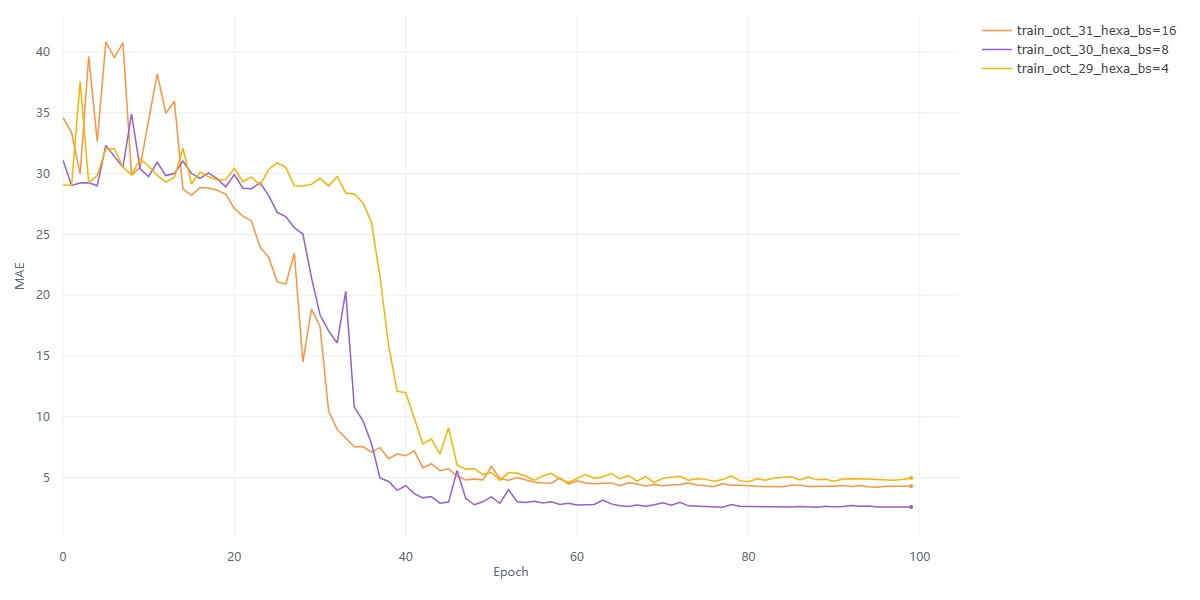
\includegraphics[width=1\linewidth]{figures/BS Valid_ MAE VS epoch.jpeg}
    \caption{Validation: MAE vs Epoch for Different Batch Sizes}
\end{figure}

\begin{table}[H]
    \centering
    \begin{tabular}{|c|c|c|c|c|}
        \hline
         Experiment Name& Batch Size & Test Loss & Test ACC & Test MAE\\
         \hline
         train oct 29 hexa bs=4& 4 & 2.719 & 0.9533 & 4.668\\
         \hline
         train oct 30 hexa bs=8& 8 & 2.592 & 0.9779 & 2.937\\
         \hline
         train oct 31 hexa bs=16& 16 & 2.638 & 0.9679 & 3.796\\
         \hline
    \end{tabular}
    \caption{Final Test Result of Different Batch Sizes}
\end{table}



\section*{The DL Experiment Result of Different Sound Source Status and SNR Ranges}
\addcontentsline{toc}{section}{The Experiment Result of Different Sound Source Status and SNR Ranges}
\begin{figure}[H]
    \centering
    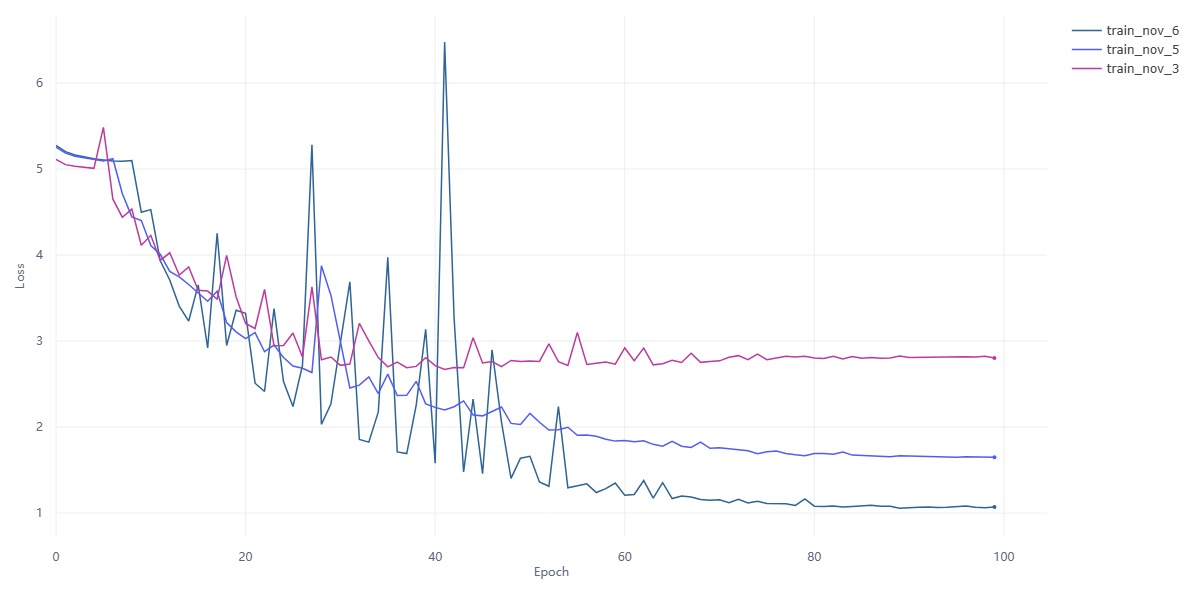
\includegraphics[width=1\linewidth]{figures/StatusSNR Valid_ Loss VS epoch.jpeg}
    \caption{Validation: Loss vs Epoch for Different Status and SNR Ranges}
\end{figure}
\begin{figure}[H]
    \centering
    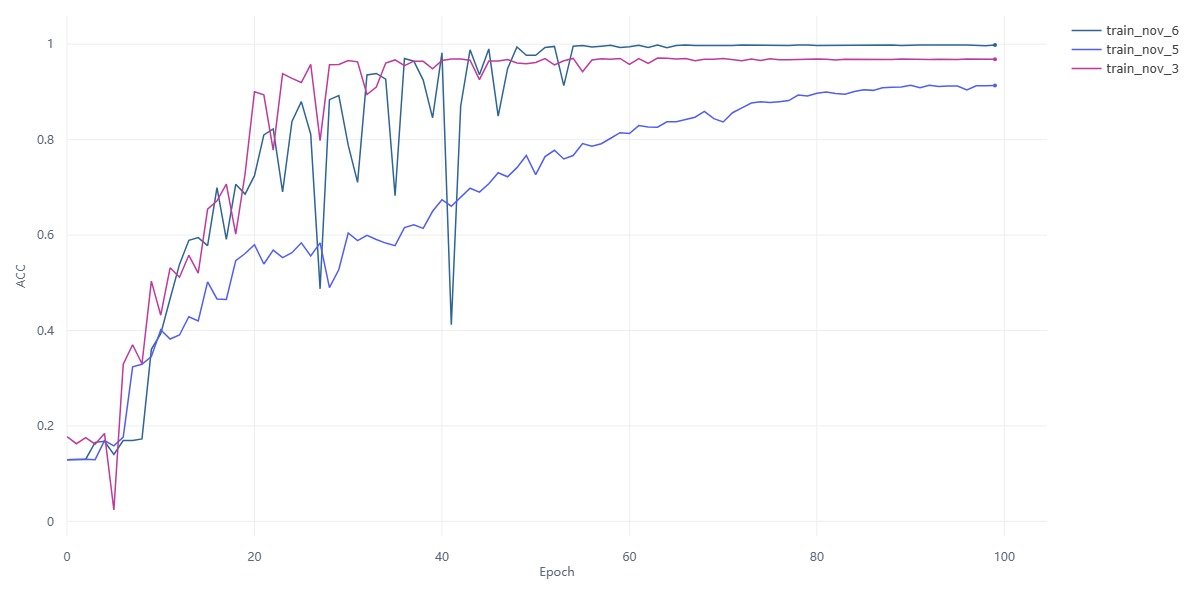
\includegraphics[width=1\linewidth]{figures/StatusSNR Valid_ ACC VS epoch.jpeg}
    \caption{Validation: ACC vs Epoch for Different Status and SNR Ranges}
\end{figure}
\begin{figure}[H]
    \centering
    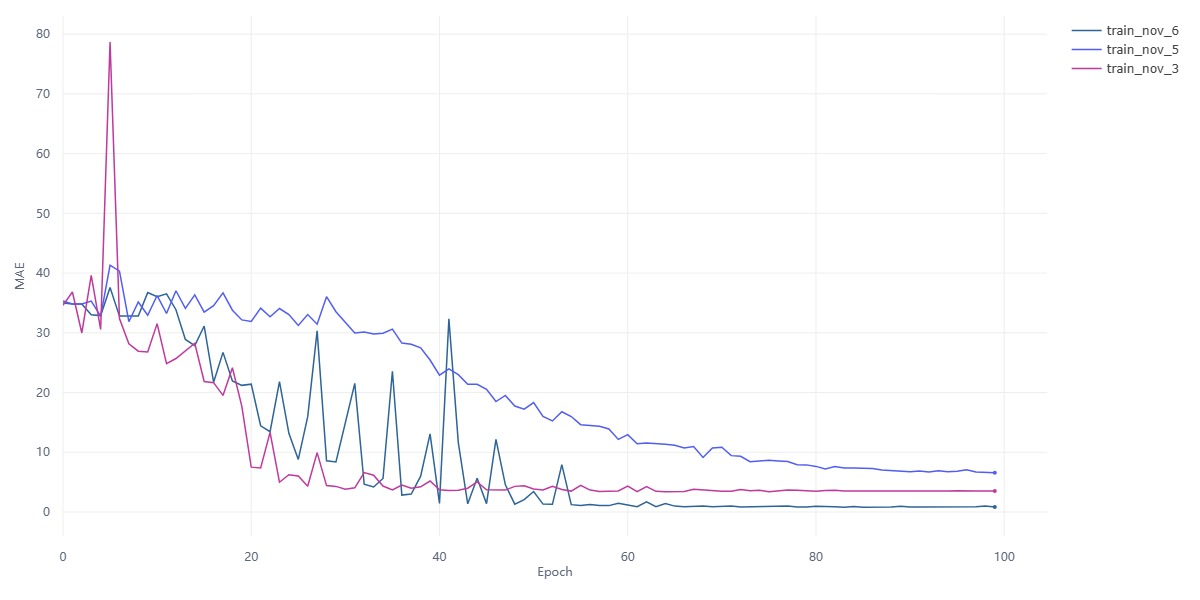
\includegraphics[width=1\linewidth]{figures/StatusSNR Valid_ MAE VS epoch.jpeg}
    \caption{Validation: MAE vs Epoch for Different Status and SNR Ranges}
\end{figure}
\begin{table}[H]
    \centering
    \begin{tabular}{|c|c|c|c|c|c|}
        \hline
         Experiment Name& Status & SNR (range in \(db\)) & Test Loss & Test ACC & Test MAE\\
         \hline
         train nov 3 & Mobile & \([-5, 15]\) & 2.731 & 0.9740 & 3.381\\
         \hline
         train nov 5 & Static & \([-5, 15]\) & 1.597 & 0.9145 & 5.568\\
         \hline
         train nov 6 & Static & \([1, 10]\) & 1.043 & 0.9988 & 0.789\\
         \hline
    \end{tabular}
    \caption{Final Test Result of Different Status and SNR Ranges}
\end{table}


\section*{The DL Experiment Result of Different SNRs}
\addcontentsline{toc}{section}{The Experiment Result of Different SNRs}
\begin{figure}[H]
    \centering
    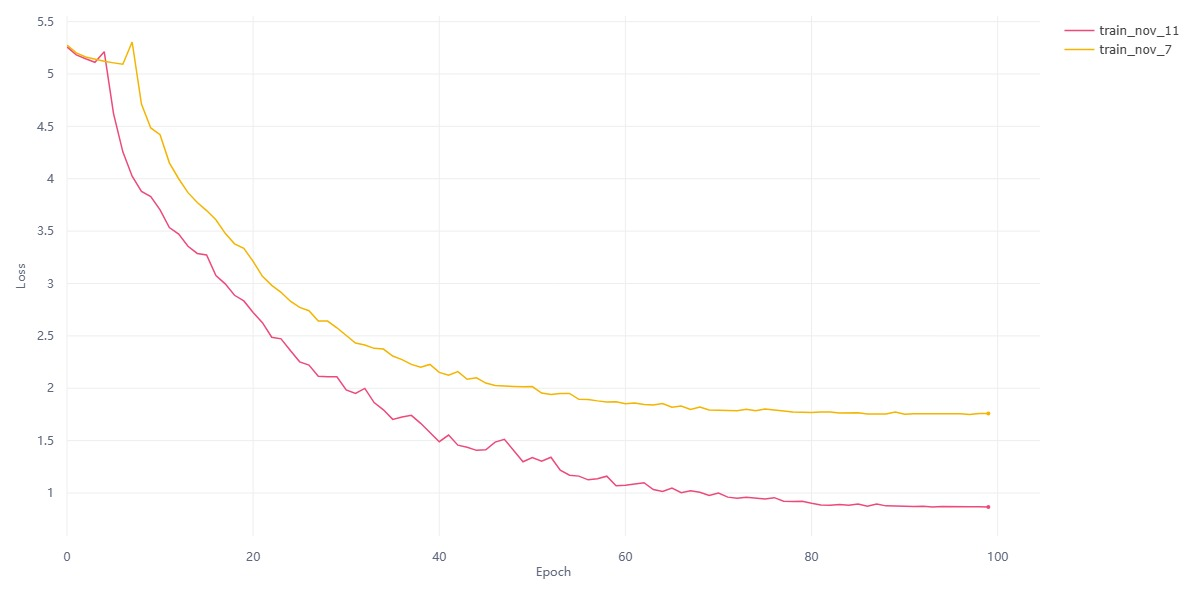
\includegraphics[width=1\linewidth]{figures/SNRs Valid_ Loss VS epoch.jpeg}
    \caption{Validation: Loss vs Epoch for Different SNRs}
\end{figure}
\begin{figure}[H]
    \centering
    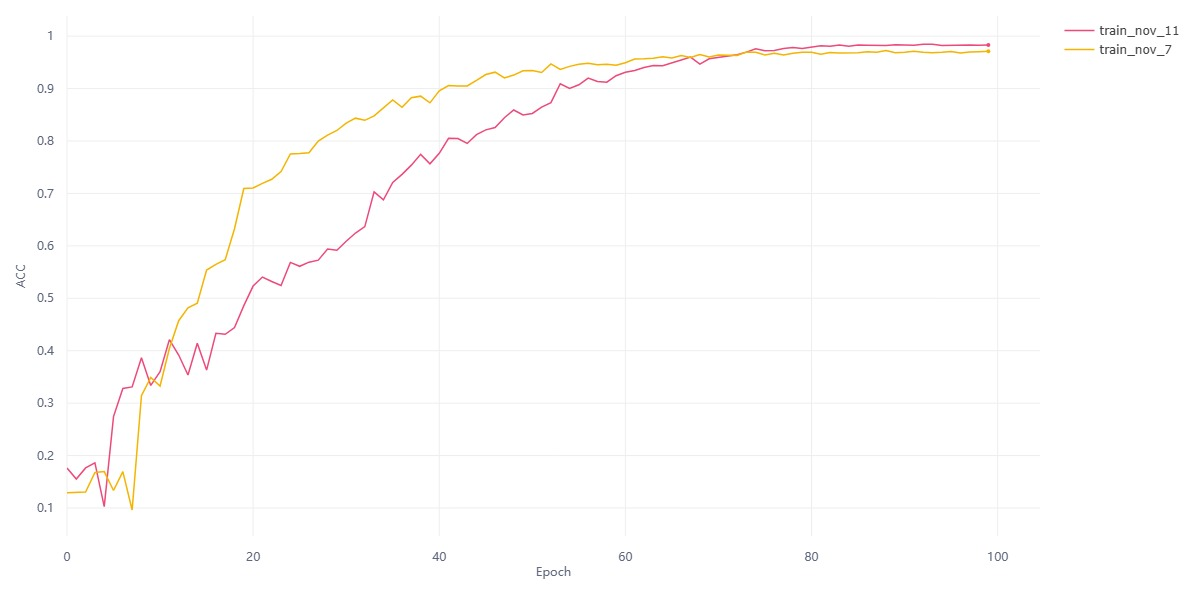
\includegraphics[width=1\linewidth]{figures/SNRs Valid_ ACC VS epoch.jpeg}
    \caption{Validation: ACC vs Epoch for Different SNRs}
\end{figure}
\begin{figure}[H]
    \centering
    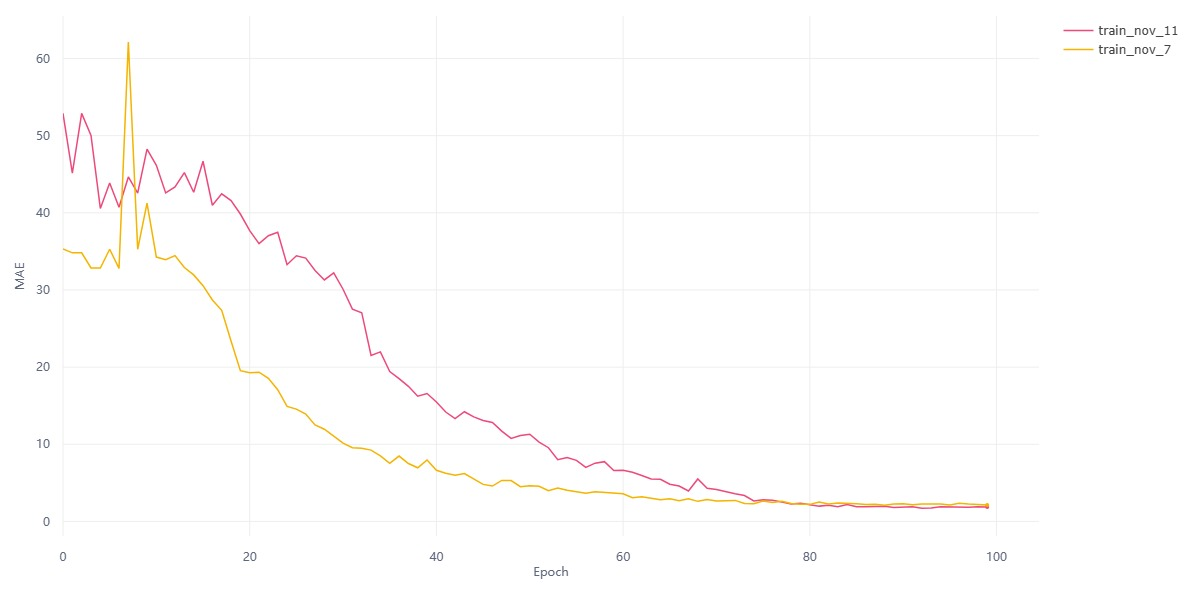
\includegraphics[width=1\linewidth]{figures/SNRs Valid_ MAE VS epoch.jpeg}
    \caption{Validation: MAE vs Epoch for Different SNRs}
\end{figure}
\begin{table}[H]
    \centering
    \begin{tabular}{|c|c|c|c|c|c|}
        \hline
         Experiment Name& SNR (range in \(db\)) & Test Loss & Test ACC & Test MAE\\
         \hline
         train nov 7 & \([1, 10]\) & 1.724 & 0.9723 & 2.198\\
         \hline
         train nov 1 & \([30, 40]\) & 0.8746 & 0.9772 & 2.38\\
         \hline
    \end{tabular}
    \caption{Final Test Result of Different SNRs}
\end{table}